\documentclass[11pt]{article}

\usepackage{fullpage}
\usepackage[english]{babel}
\usepackage[utf8]{inputenc}
\usepackage{amsmath}
\usepackage{graphicx}
\usepackage[colorinlistoftodos]{todonotes}
\usepackage{array}
\usepackage{longtable}


\begin{document}
\noindent
\large\textbf{Alvin Nguyen, Devin Stoen} \hfill \textbf{EE-393 Technical Writing} \\
\normalsize Quiz Section AB \hfill Professor Bade \\
\today \hfill Julianne Dorothy Peeling \\

\begin{center}
\section*{Solar Generators for Children in Africa}
\end{center}

\section*{Problem Statement}
Computers and laptops are a huge help in educating children. However, you need power in order to run the computers/laptops at the school.

\section*{Solution}
So we intend to help provide that power by using affordable power generators. These power generators will be powered by solar panels. 

\section*{Product Specifications (Visuals)}
\begin{center}
\begin{tabular}{|c|c|}
\hline
size & Power generator: 7” x 12” x 7”\\&Solar panels: 3’ x 2’ x 1”\\
\hline
weight & 14.5lbs\\
\hline
Cost & \$400-500\\
\hline
\end{tabular}

Table 1. Design Specs

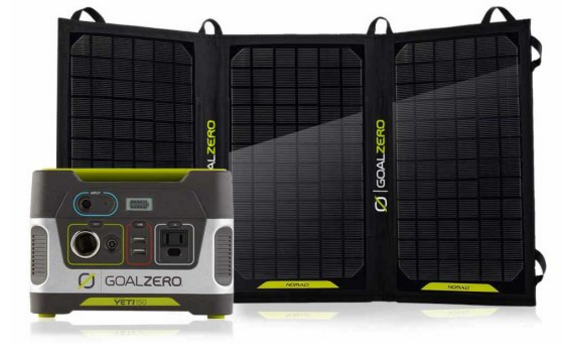
\includegraphics[scale=0.5]{solar}

Figure 1. Generator and Solar Panels
\end{center}

\section*{Conclusion (Why should you be rewarded)}
Modern Science and technology is heavily dependent on electrical tools and implements. To use these things, they need to be powered. So, for the children of Africa to learn, they need power. We can supply that power with our affordable and portable power generator.

\end{document}
